\addcontentsline{toc}{chapter}{Разработка и исследование преобразователя силы на основе Velostat}

\textbf{\underline{Третья глава}} посвящена разработке и исследованию преобразователя силы на основе Velostat. Задача -- измерить характеристики материала для случаев, когда площадь приложения силы меньше, чем площадь активной части сенсора.

Входными данными являются показания разработанного преобразователя и значение реально приложенной нагрузки. На выходе получается разница между нормальным значением с датчика и реальной нагрузкой.

Для решения задачи проводилось два эксперимента. В \textbf{статическом эксперименте} решалась задача определения коэффициентов для математической модели преобразователя \eqref{eq:velostat_eqn}. В рамках эксперимента на сенсор прикладывалась известная нагрузка на 60 секунд \pic{fig:tikz_exp/tikz_pictures6.png}. Для решения задачи регрессии использовался робастный нелинейный алгоритм наименьших квадратов \pic{fig:least_square_model.png}.

\begin{align}
    \label{eq:velostat_eqn}
    V_{out} = V_0 + p[k_p + k_e(1-e^\frac{-(t-t_0)}{\tau_{res}})](1-e^{-\frac{A}{p}}) \\
    k_p = A_1e^{-A_2p}; \tau_{res} = B_0 + B_1e^{-\frac{p}{B_2}}
\end{align}
где,  $V_0$- начальное напряжение; $p,\ A_i,\ B_i,\ \tau_{res},\ k_i$  - настраиваемые константы; $t$ - текущее время; $t_0$ - время начала нажатия.


\begin{figure}[h]
    \begin{subfigure}[t]{0.35\textwidth}
        \centering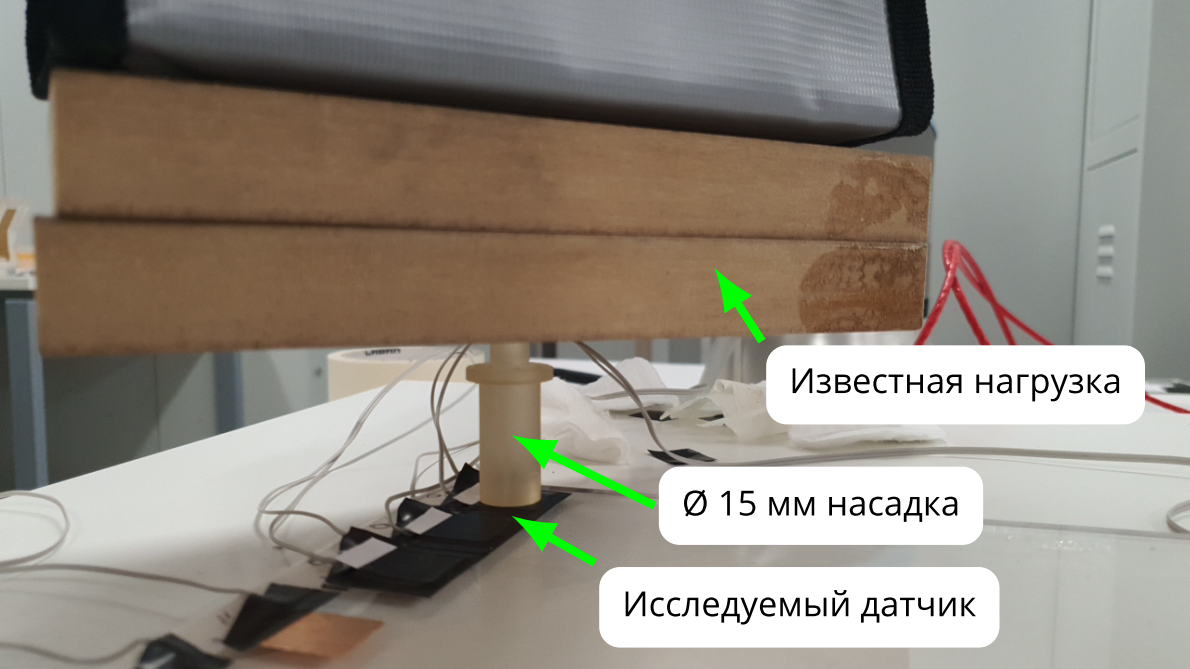
\includegraphics[height=3cm,width=1\textwidth,keepaspectratio]{tikz_exp/tikz_pictures6.png}
        \caption{Стенд для эксперимента}
        \label{fig:tikz_exp/tikz_pictures6.png}
    \end{subfigure}
    \begin{subfigure}[t]{0.54\textwidth}
        \centering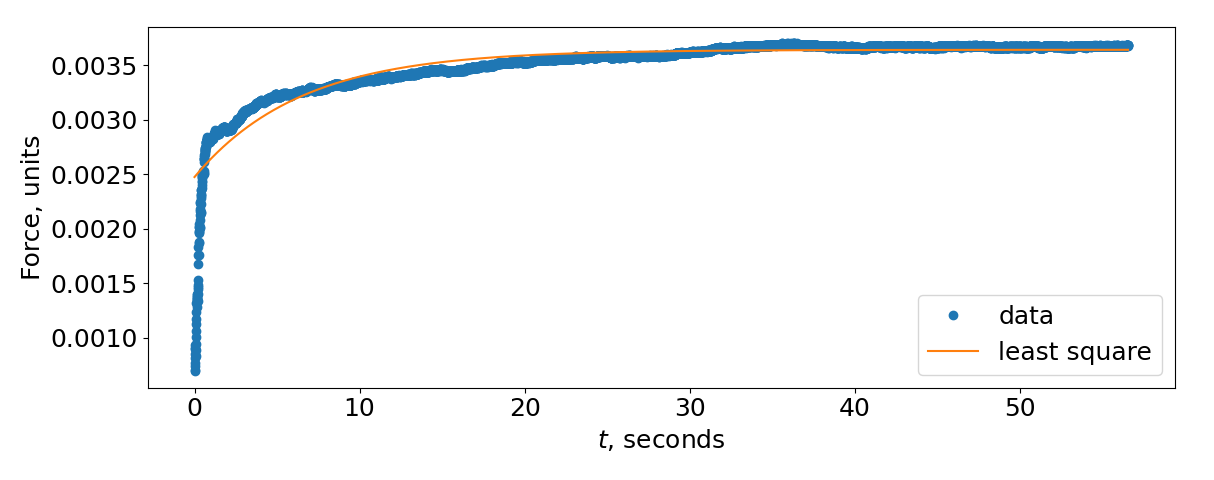
\includegraphics[height=3cm,width=1\textwidth,keepaspectratio]{least_square_model.png}
        \caption{Результаты статического эксперимента}
        \label{fig:least_square_model.png}
    \end{subfigure}

\caption{Статический эксперимент}
\label{fig:static_expp}
\end{figure}

В \textbf{динамическом эксперименте} определялось влияние показаний сенсора в зависимости от положения площадки контакта. Для этого преобразователь представлен в виде матрицы $4 \times 4$ \pic{fig:sensor_grid}. Манипулятор нажимает на преобразователь с одинаковым давлением на протяжении всех экспериментов в различные позиции на преобразователе, используя последовательно пять насадок. Роботизированный стенд, представлен на рисунке \ref{fig:exp_standd}.


\begin{figure}[h]
    \begin{subfigure}[t]{0.45\textwidth}
        \centering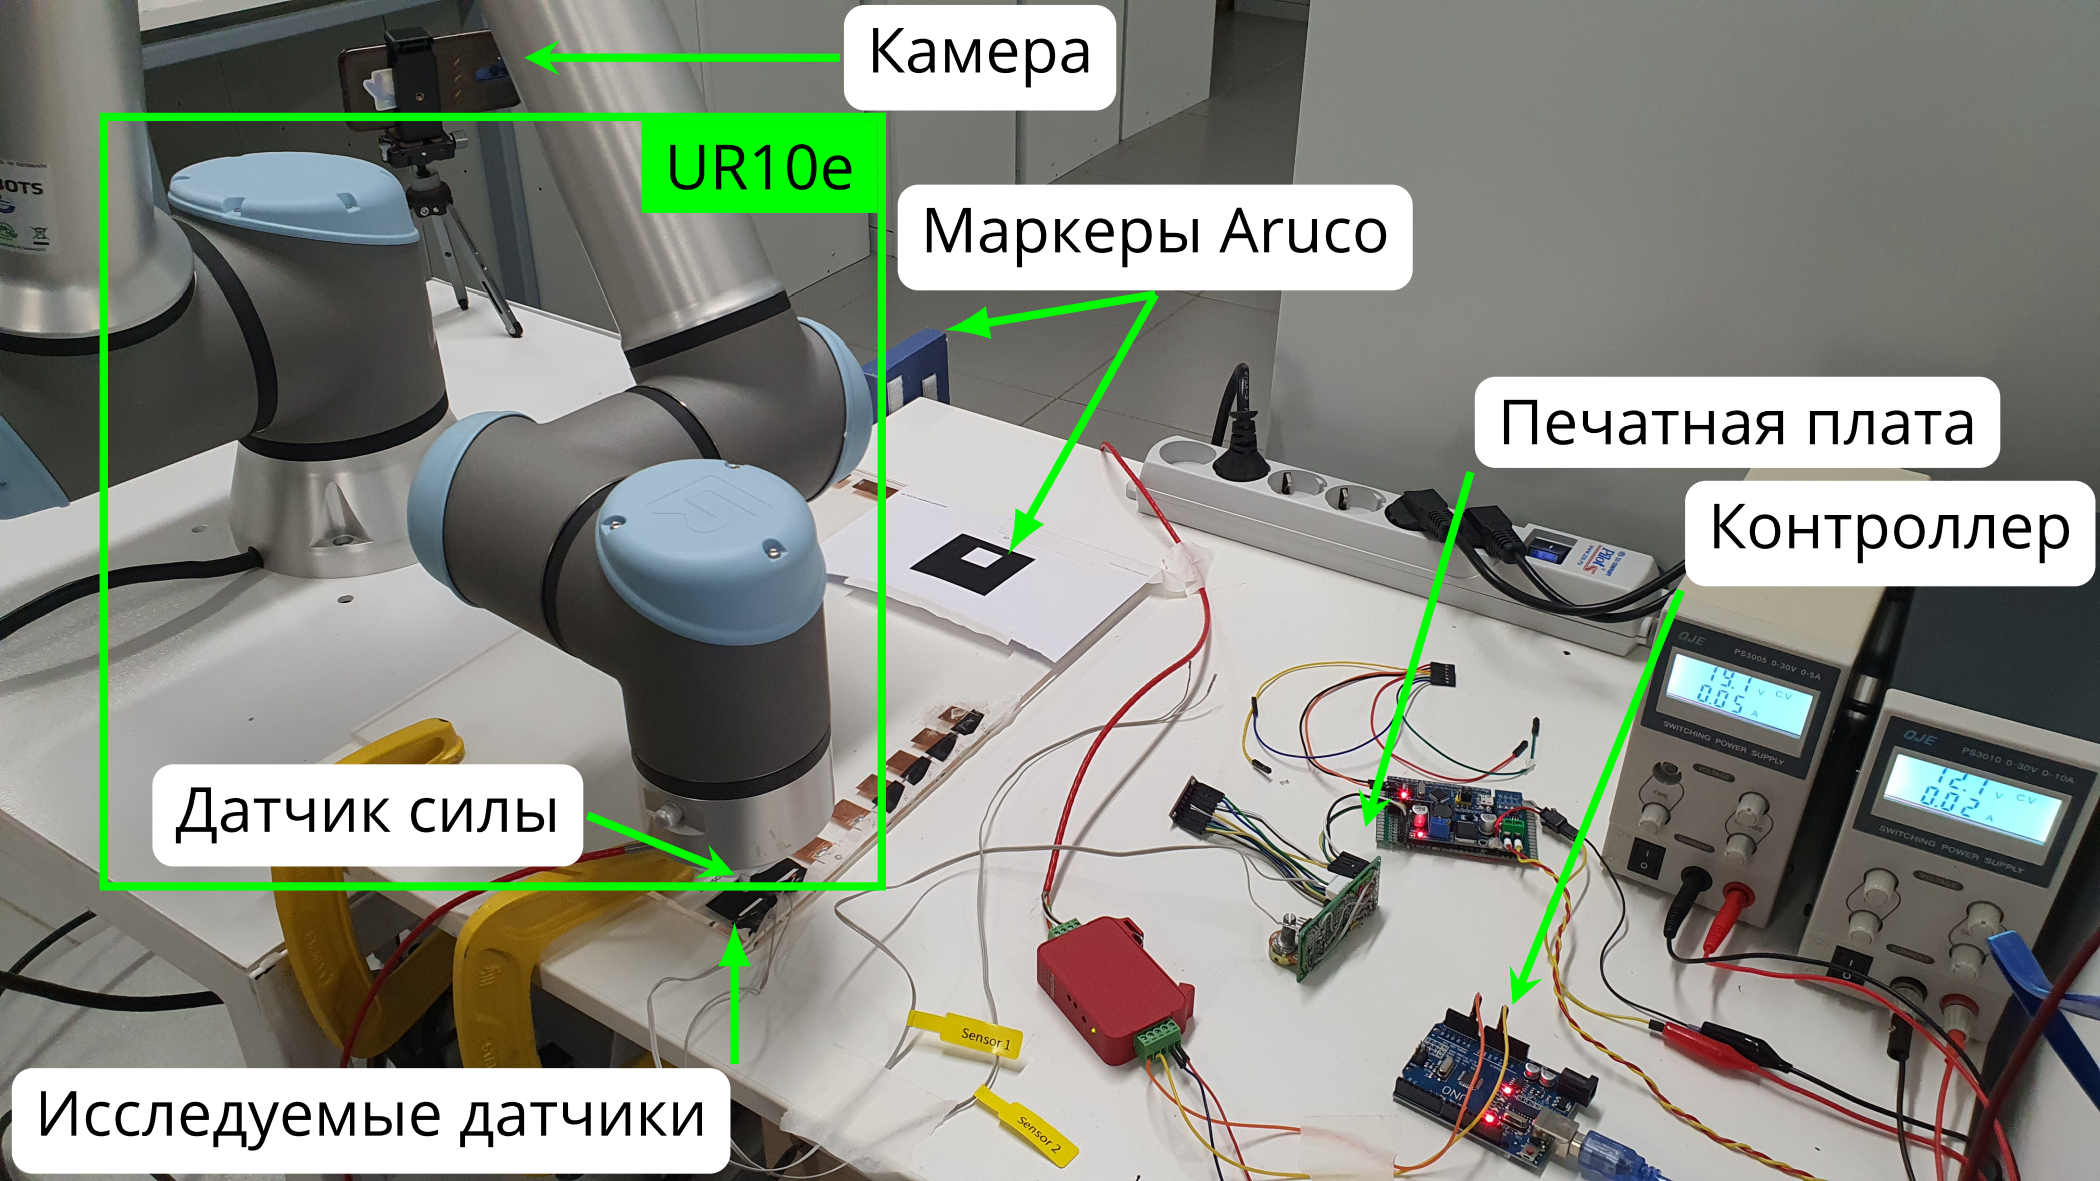
\includegraphics[height=3cm,width=1\textwidth,keepaspectratio]{tikz_exp/tikz_pictures7.png}
        \caption{Разработанный экспериментальный стенд}
        \label{fig:exp_standd}
    \end{subfigure}
    \begin{subfigure}[t]{0.24\textwidth}
        \centering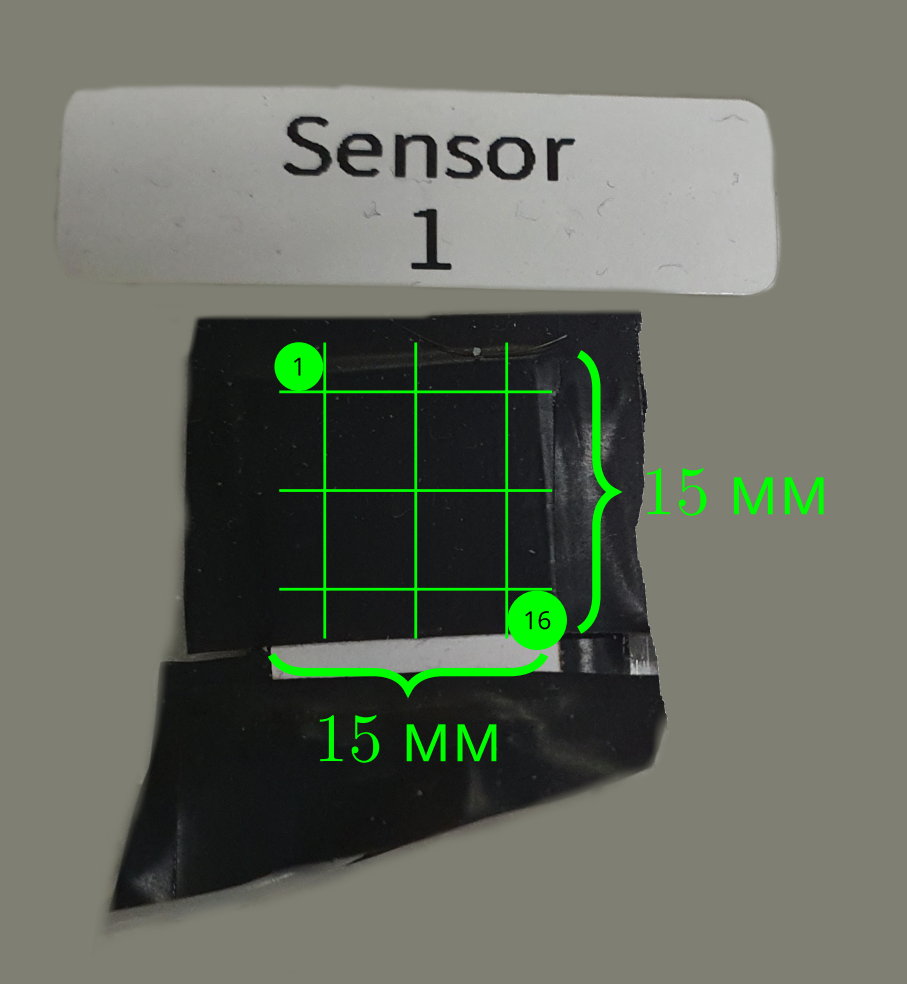
\includegraphics[height=3cm,width=1\textwidth,keepaspectratio]{tikz_exp/tikz_pictures5.png}
        \caption{Сенсор представлен \\ как $4\times4$ сетка}
        \label{fig:sensor_grid}
    \end{subfigure}
    \begin{subfigure}[t]{0.3\textwidth}
        \centering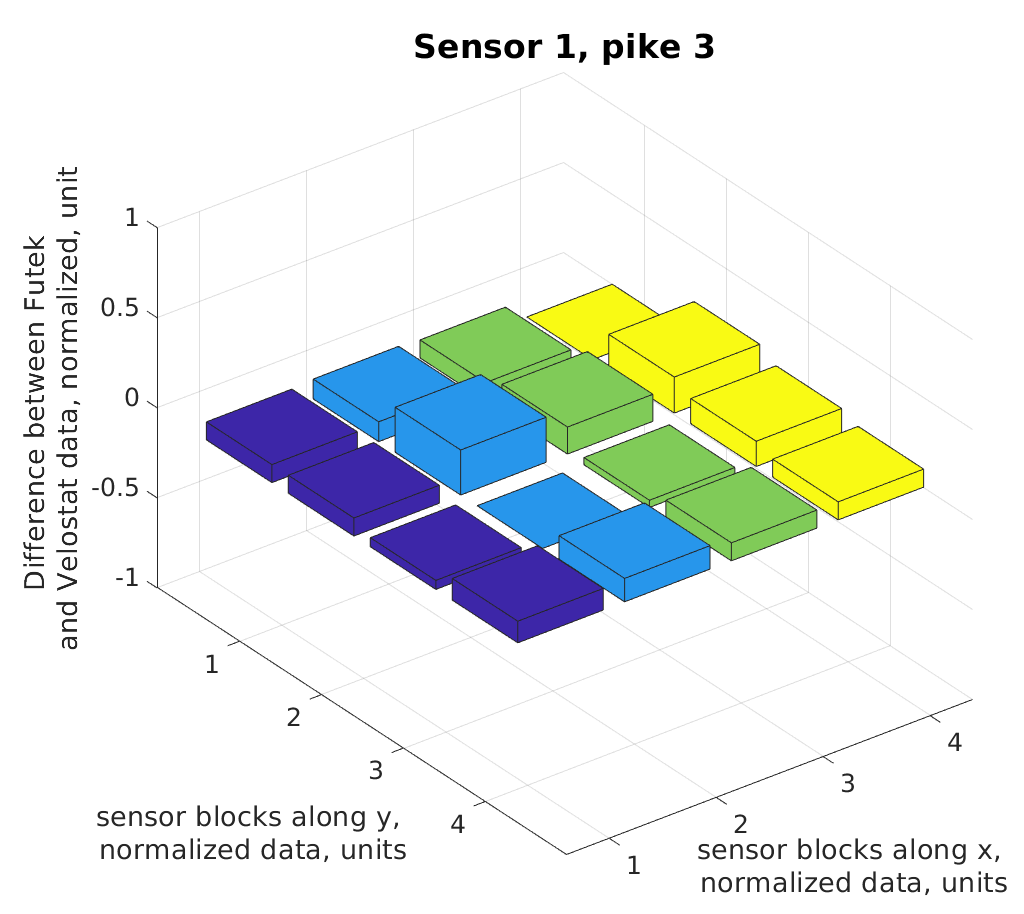
\includegraphics[height=3cm,width=1\textwidth,keepaspectratio]{sens1_pike3.png}
        \caption{Зависимость погрешности датчика}
        \label{fig:sens1_pike3}
    \end{subfigure}
    \caption{Представление места нажатия инструментом сенсора и сам инструмент}
\end{figure}


% Результаты распределения ошибок по площади сенсора при взаимодействии с насадками разных размеров \pic{fig:dynamics_exp}. Ошибки определялись как разница между нормализованными показаниями калиброванного сенсора силы Futek и исследуемого преобразователя на базе Velostat.

% \begin{figure}[ht]
%     \begin{subfigure}{0.49\textwidth}
%         \centering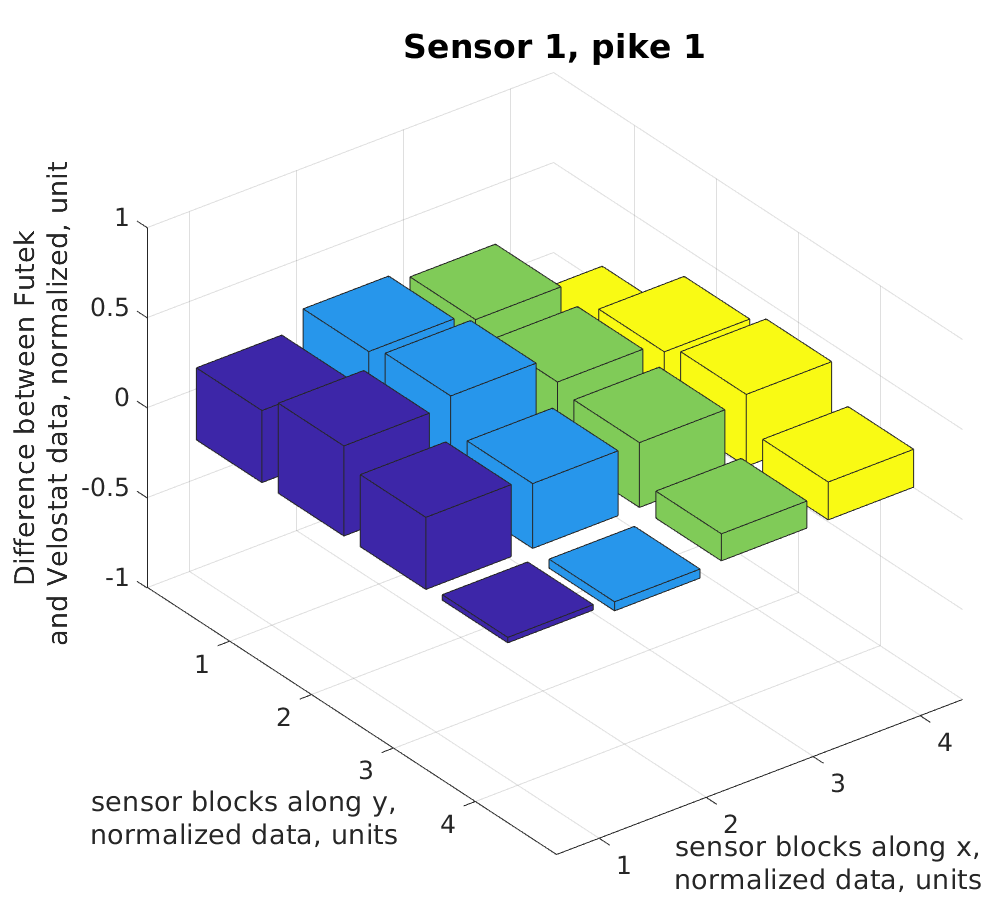
\includegraphics[height=5cm,width=1\textwidth,keepaspectratio]{sens1_pike1.png}
%         \caption{Диаметр насадки равный 2 мм }
%         \label{fig:sens1_pike1}
%     \end{subfigure}
%     \begin{subfigure}{0.49\textwidth}
%         \centering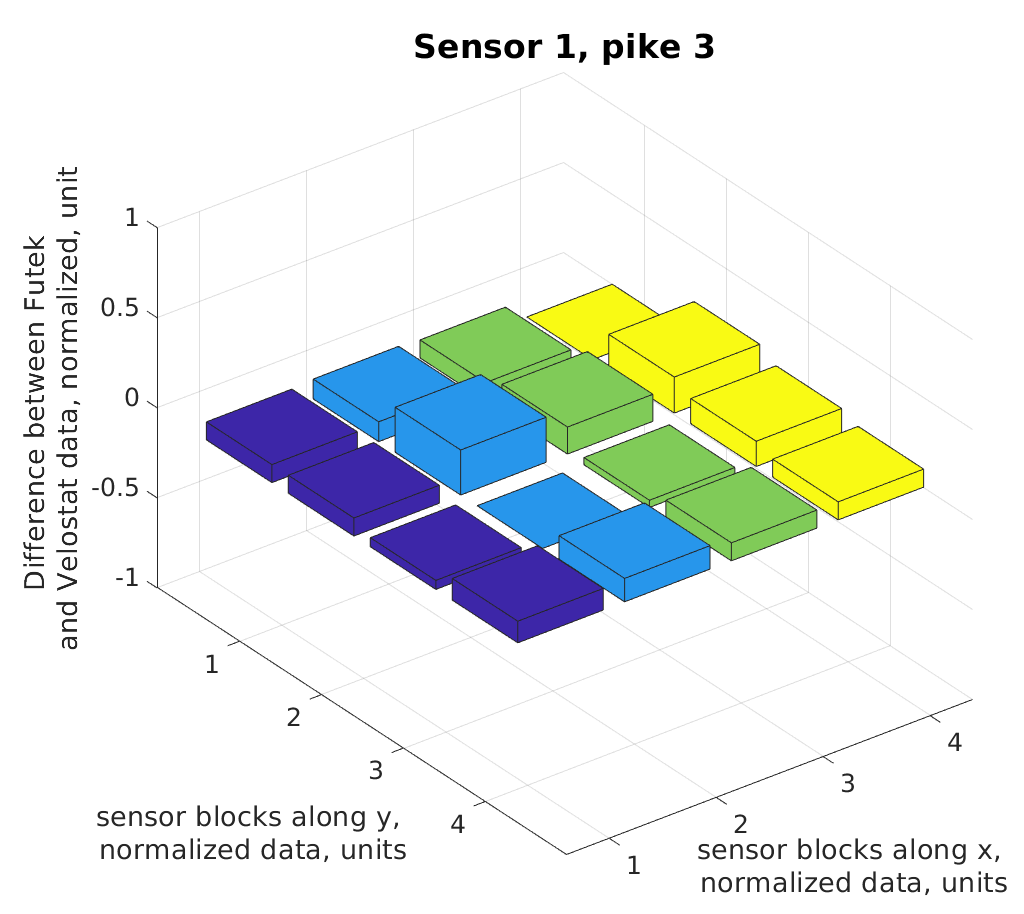
\includegraphics[height=5cm,width=1\textwidth,keepaspectratio]{sens1_pike3.png}
%         \caption{Диаметр насадки равный 8 мм }
%         \label{fig:sens1_pike3}
%     \end{subfigure}
%     \caption{Динамический эксперимент}
%     \label{fig:dynamics_exp}
% \end{figure}

Результатом исследования является зависимость, что характеристики преобразователя удовлетворяют требованиям к системе тактильного восприятия шагающего робота, когда ожидаемый размер площади контакта превышает 25 процентов площади преобразователя.
